\documentclass{thesisreport}
\usepackage{todonotes}
\usepackage{parskip}
\usepackage{graphicx}
\usepackage{float}
\usepackage{multicol} %aggiunto da me
\usepackage{enumitem}
\usepackage{caption}

\documentclass[main.tex]{subfiles}
\begin{document}
\begin{center}
\begin{longtable}{ |p{0.8cm}p{6.8cm}|p{0.8cm}p{6.8cm}|  }
 \hline
 \multicolumn{4}{|c|}{Instrumental ADL} \\
 \hline
 \textit{\textbf{Score}} & \textit{\textbf{Activities}} & \textit{\textbf{Score}} & \textit{\textbf{Activities}}\\
 \hline
 \vspace{0.15cm} & & &\\
 
  & \textbf{A. Ability to use telephone}  & & \textbf{E. Laundry}  \\
  
 1 & A.1 Operates telephone on own initiative; looks up and dials numbers, etc. & 1  & E.1 Does personal laundry completely \\
 
 1 & A.2 Dials a few well-known numbers & 0 &  E.2 Launders small items; rinses stockings, etc.\\
 
 1    & A.3 Answers telephone but does not dial & 0 & E.3 All laundry must be done by others.\\
 
 0 & A.4 Does not use telephone at all. & & \\
 
 \vspace{0.15cm} & & &\\

 & \textbf{B. Shopping} & & \textbf{F. Mode of Transportation} \\
 
 1 & B.1 Takes care of all shopping needs independently & 1 & F.1 Travels independently on public transportation or drives own cars. \\
 
 0 & B.2 Shops independently for small purchases & 1 & F.2 Arrange own travel via taxi, but does not otherwise use public transportation.\\
 
 0 & B.3 Needs to be accompanied on any shopping trip. & 1 & F.3 Travels on public transportation when accompanied by another.\\
 
 0 & B.4 Completely unable to shop. & 0 & F.4 Travel limited to taxi or automobile with  assistance of another.\\
 
 & & 0 & F.5 Does not travel at all.\\
 
 \vspace{0.15cm} & & &\\

 & \textbf{C. Food Preparation} & & \textbf{G. Responsibility for own medications}\\
 
 1 & C.1 Plans, prepares and serves adequate meals independently & 1 & G.1 Is responsible for taking medication in correct dosages at correct time.\\
 
 0 & C.2 Prepares adequate meals if supplied with ingredients & 0 & G.2 Takes responsibility if medication is prepared in advance in separate dosage.\\
 
 0 & C.3 Heats, serves and prepares meals or prepares meals but does not maintain adequate diet. & 0 & G.3 Is not capable of dispensing own medication.\\
 
 0 & C.4 Needs to have meals prepared and served. & & \\
 
 \vspace{0.15cm} & & &\\
  
 & \textbf{D. Housekeeping} & & \textbf{H. Ability to Handle Finances}\\ 
 
 1 & D.1 Maintains house alone or with occasional assistance (e.g. “heavy work domestic help”) & 1 & H.1 Manages financial matters independently (budgets, writes checks, pays rent, bills goes to bank), collects and keeps track of income.\\
 
 1 & D.2 Performs light daily tasks such as dish-washing, bed making & 1 & H.2 Manages day-to-day purchases, but needs
help with banking, major purchases, etc.\\

 1 & D.3 Performs light daily tasks but cannot maintain acceptable level of cleanliness. & 0 & H.3 Incapable if handling money.\\
 
 1 & D.4 Needs help with all home maintenance tasks. & & \\
 0 & D.5 Does not participate in any housekeeping tasks. & &\\
  
 \hline
\end{longtable}
\captionof{table}{Instrumental Activities of Daily Living Scale \cite{lawton1970assessment}.}
\label{tab:IADL}

\end{center}
\end{document}

\begin{document}

\thispagestyle{empty}

\def\lskip{\vspace{0.5cm}}


\begin{tabular}{p{7cm}p{10cm}}
ÉCOLE CENTRALE DE NANTES
&
\raggedleft UNIVERSITÀ DEGLI STUDI DI GENOVA	% for EMARO students
\end{tabular}

\vspace{2cm}

% EMARO students
\begin{center} \large\sc MASTER ERASMUS MUNDUS \\ \normalsize{EMARO+ ``European Master in Advanced Robotics''} \end{center}


\begin{center}
	2018 / 2019\\
	\lskip
	Master Thesis Report
	\lskip
	
	Presented by \lskip 
	
	Tommaso Elia \lskip
	
	28/12/2018 \lskip\lskip
	
	{\Large \textbf{Dialogue-based interaction processes with smart homes and companion robots}}
	
	\vfill

Jury \lskip
		
	\end{center}
	


\begin{tabular}{p{3cm}p{6cm}p{6cm} }
 President: & Name & Position (Institution) \\ & & \\ 
 Evaluators: & Name & Position (Institution) \\
	      & Name & Position (Institution) \\ 
	      & Name & Position (Institution) \\ & & \\  & & \\ 
  Supervisor(s):  & Fulvio Mastrogiovanni & Assistant Professor (UNIGE)\\
		  & Enrico Reboscio & Project Menager (DotVocal S.r.l.) \\
		  & Renato Zaccaria & Assistant Professor (UNIGE) \\
(EMARO)  & Co-supervisor from M1 & Position, M1 institution 
\end{tabular}

\lskip

\begin{flushleft}
 Laboratory: Laboratoire des Sciences du Numérique de Nantes LS2N
\end{flushleft}

\newpage
\thispagestyle{empty}
\null
\newpage
\addtocounter{page}{-1}
\pagestyle{fancy}
  
 
\section*{Abstract}
   
 Do not forget to check each reference while importing in your Bibtex file.
 Especially, IEEExplore export may lead to ill-formatted conference name like \emph{Robotics and Automation, 
 IEEE International Conference on}.
 
 \newpage
 
 %\section*{Acknowledgements}
 %\newpage
 
\section*{Notations}
 
 \newpage
 
 \section*{Abbreviation}
 
 \begin{tabular}{p{2cm}p{12cm}}
 ADL & Activities of Daily Living\\
 AAL & Ambient Assisted Living \\
 IADL & Instrumental Activities of Daily Living \\
 DS & Dempster - Shafer \\
 DL & Description Logic \\
 SWRL & Semantic Web Rule Language\\
 OWL & Ontology Web Language\\
 EMS & Emergency Medical Services \\
 AR & Activity Recognition \\
 IOT & Internet of Things \\
 ML & Machine Learning \\
 TBox & Terminological Box \\
 ABox & Assertional Box \\
 GUI & Graphical User Interface \\
 \end{tabular}
 
 \newpage
 
 \listoffigures
 
 \listoftables
 
 \tableofcontents
 
 
 \chapter{Introduction}
 %\addcontentsline{toc}{chapter}{Introduction}	 % non-numbered chapters do not appear in table of contents by default

\section{Motivation}
  The demographic growth along with progress of medical technologies results in an increase of elderly population. Indeed in most of the industrialized countries the demographic and social trends have led to greater elderly burden among the population, and that situation critically increases health care demand. Therefore, emergency medical services, public and private health care and patients are subject to more and more stress. 
  In particular, the raising of the average age of the population means higher incidence of chronic diseases that require frequent health assistance and can result in disability and/or lost of independence and deeply affecting health economy for the increasing cost of care. Moreover, if there is a suboptimal management of these diseases there is also an increasing use of Emergency Medical Service (EMS), often avoidable.
 
 In the district of Kaiserslautern, Germany, a significant study was conducted showing that 44\% of Emergency Medical Services (EMS) are dedicated to elderly above 70 years of age \cite{kleinberger2007ambient}.
 	\begin{figure}[H]
		\centering
		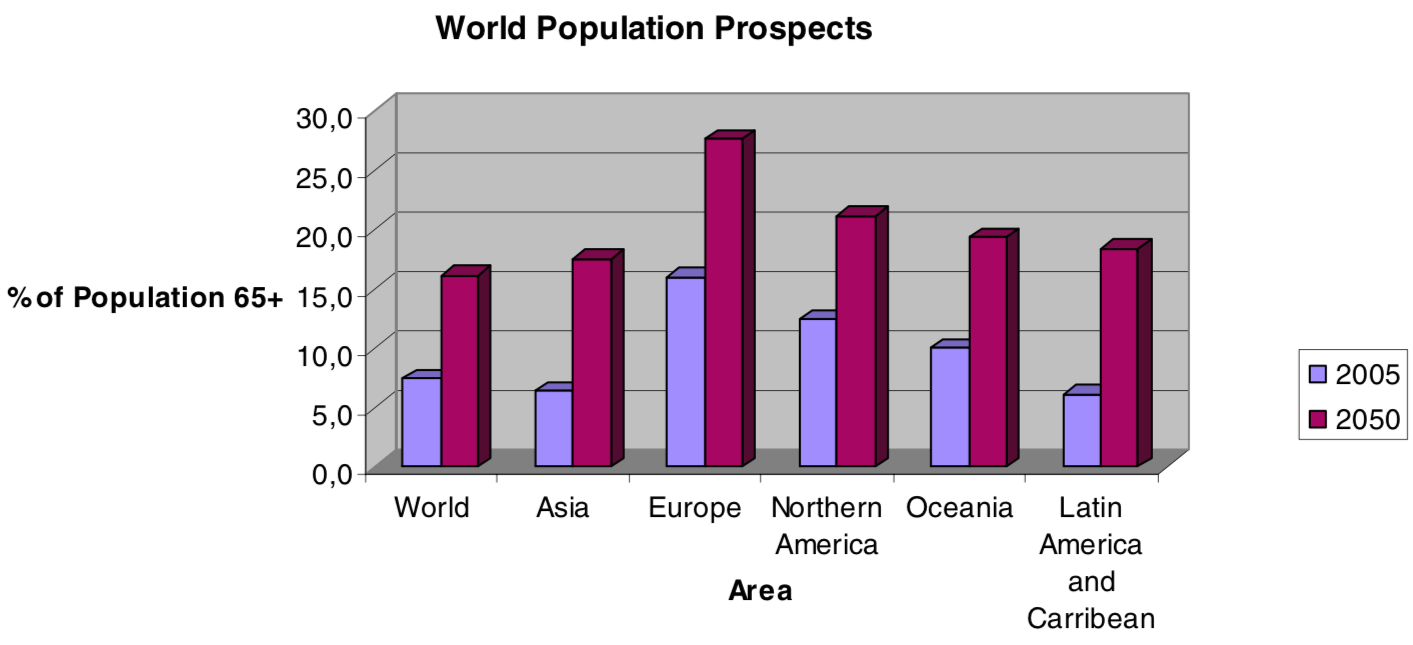
\includegraphics[width=15cm]{Thesis/data/populationProspect.png}
		\caption{\small{Demographical Change according to the United Nations World Population Prospects \cite{kleinberger2007ambient}}}
		\label{fig:populationProspect}
	\end{figure}
 All these elements highlight the increasing cost of health care, the underperforming management of resources and the decline of service quality.
 
 \parskip  \parskip
 
 The Ambient Intelligence technologies help to cope with trends, providing proactive and conscious assistance and supporting the autonomy of the elderly, indeed Assisted Living solutions not only can reduce the costs of managing and monitoring older people but can also offer better \textit{quality of life} \cite{kleinberger2007ambient}.
 
 \section{Context of the Study}
  To guarantee an improved quality of life it is necessary to ensure that the Activities of Daily Living (ADL) are correctly and regularly performed by the assisted \cite{buoncompagni2017towards}.
 
 ADL are defined as daily activities related to motion, rest, nutrition, and personal hygiene, which are a qualitative indicator of person’s wellbeing, determining their quality of life and level of independence \cite{buoncompagni2017towards}. 
 
 At this purpose, in literature the term smart home is used as synonymous of a home that is context-aware. Context awareness has been defined as: ``having information that can be used to characterize the situation of an entity, where an entity can be a person, place, physical or computational object that is considered relevant to the interaction between a user and an application, including the user and applications themselves" \cite{abowd1999towards}.  

 Today, the idea of smart home is deeply changed, especially due to giant stride of the technologies that support it, giving the possibility to create increasingly complex and sophisticated architectures of intelligent environments. At this regard, in the domain of assistive robots and IOT (Internet of Things) field has taken a leading role, also for technological advances in the miniaturization and increased battery life of different types of sensors \cite{phdthesis} \cite{nakashima2009handbook}.
 
 For an easier and immediate comprehension of the possibilities possible by this type of technology, let's have a look to some interesting scenarios that facilitate independence of the elderly individuals:
 \begin{itemize}
     \item \textit{Scenario 1}: The geriatrician with the task of monitoring the health status of elderly could monitor the quality of the patient's sleep through wearable devices or pressure sensors positioned at the base of the bed, visualizing the pattern of sleep during the night;
     \item \textit{Scenario 2}: The system could monitor the daily activities such as getting out of bed, washing and having breakfast etc. and if the patient, for example, stop eating the system warns the geriatrician;
     \item \textit{Scenario 3}: The elder after having woken up decides to take a walk, he puts on his coat and as soon as he crosses the threshold the system realizes that it will  probably rain and the elder has not taken the umbrella risking thus to fall ill. Then the system alerts him via a notification on the wearable device or directly via a voice interface;
     \item \textit{Scenario 4}: The elderly person who is alone at home  and is heading to the bathroom to wash. The system detects his presence in the bathroom and also receives an unclear signal from the wearable he wears that could represent a fall by the elderly. To be certain of the elderly safety, the system could verify it  in two ways: it could ask the elderly about his state through a voice interface or it could send a robot 'companion' to check the situation (for example through image analysis - ML);
 \end{itemize}
 
 Smart systems are a very useful reality but it is important not to forget the value of human-human interaction because we do not want that the elderly who are already at a risk of isolation, are further isolated from others, more than before.
 
 \section{Objectives}
 There are many difficulties and challenges in the smart environment, many of them linked to the importance of the general acceptance of the system by the elderly, allowing them to learn how to get used to the assistance provided. For this reason, the system must meet the following user interface requirements:
 \begin{itemize}
     \item Adaptability:  the systems need to adapt themselves to the context at runtime;
     In order to guarantee the best possible service, the system adapts itself according to the situation, for example by scaling down the complexity of the interface in case of emergencies to reduce the cognitive load;
     To do this, the system must be able to monitor the environment around it at all times, to reason on what it perceives and then make the necessary adjustments.
     \item  Natural, anticipatory human-computer interaction: the system must provide different levels of interfaces for different types of users; in particular for the medical and assistance staff, for the operators of the manoeuvring but especially for the assisted persons whose interface must be specially designed according to the their limitations; 
     Indeed the anticipatory interfaces that proactively contact persons in certain situations are considered mandatory.
     \item Heterogeneity: the system must be able to integrate different subsystems supplied by different manufacturers, providing a unique and homogeneous user interface;
 \end{itemize}
 At the same time, however, we need to consider the medical, technological, social constraints and their consequent problems, for example the difficulties for an elderly person to adapt and understand a new technology, or the difficulties of a system to be operative from the beginning.
 
 Given the complexity and the issues typical of an ambient intelligence architecture, the aim of this thesis work is, firstly, to examine a pre-existing architecture by studying its dynamics and by pointing out the underlying strengths and weaknesses. Secondly, this study’s aim is to improve the architecture ability to acquire information also in an equivocal and ambiguous context.
 
 The architecture chosen is called Arianna+ and was developed by Teseo Srl in collaboration with the University of Genova. Arianna+ is a smart home system capable of understanding and making sense of the activities carried out by assisted people, predicting their future behaviours and suggesting personalised healthy habits.
 
 Therefore, in short, the goal is to extend Arianna's AI system as follows:
 \begin{itemize}
     \item Allow Arianna+ to intentionally acquire information when a given context or situation is equivocal, with 2 different approaches:
     \begin{itemize}
         \item By integrating a companion robot with the aim of exploiting its sensors to collect relevant data and by establishing a two-way communication with Arianna’s AI system, which is in charge of processing them and sending back to the robot specific commands;
         \item By integrating a Google Speech API based dialogue management system developed by the company Dot Vocal Srl, where each dialogue is modulated by Arianna’s AI system; 
     \end{itemize}
 \end{itemize}

 The goal is therefore to fit these characteristics in a smart home able to acquire sensory data and save them neatly relying on the context. As result of this approach, a high-level artificial intelligence is able to react also to unclear and uncertain situation, such as scenario 4, through an accurate activities’ detection from the environment and flexible and effective management of saved information.
 
 In this way, the outcome will be an improvement of the system not only functionally but also from the point of view of its usability.
 Indeed, with the integration of a voice interface and a companion robot the user will be encouraged to no longer see the house as a taciturn and hidden entity but as a pet-like to interact with or a person to talk to in case of need and beyond.
 
\section{Overview of the Thesis}
The remainder of the thesis is organized as follows. 

\quad \textit{Chapter 2} presents an overview of the main concepts and techniques adopted in the ambient intelligence field, from the choice of sensors to how and when use them, not forgetting ADL and Ontology definitions that are crucial to understand their role in the following chapters

\quad \textit{Chapter 3} presents the state of the art regarding the topics that are useful to reach our goals:
\begin{itemize}
    \item Section \ref{Arianna}: presents software architecture of Arianna+ and describes the operating mechanisms to manage data from sensors and to recognize elderly activities;
    \item Section \ref{speech}: presents the state of the art for based dialogue management system in smart environment, in particular the possible approaches and solutions that can be adopted in our case;
    \item Section \ref{companionRobot}: presents the state of the art for usage of companion robots in smart environment discussing the advantages and possible choices;
\end{itemize}

 \chapter{Background}
The objective of this chapter is to discuss briefly the different aspects that concern smart environment systems:
\begin{itemize}
    \item The types of sensors that an intelligent box should be equipped with;
    \item Possible context models to represent a given context based on sensory information;
    \item What are the ADL and how to recognize them;
    \item How to guarantee the reliability of the recognition;
\end{itemize}

 \section{Sensoring}
 An architecture able to monitor these kind of activities can provide very useful information about human behaviour to Human-Robot interaction or cooperation in smart environments \cite{bruno2014public}.  
 
%  In literature it is possible to distinguish two different approaches of monitoring: (A) one is based on heterogeneous sensor distributed in an area used to deduce the state of the person inside a context \cite{aggarwal2011human}; (B) the other achieves the information from the wearable devices which are sensors located on the person body that are able to detect its movements and vital signs \cite{bao2004activity}. 
%  Therefore we can differentiate two different pivotal concepts:
% \begin{enumerate}[label=\alph*)]
%     \item to monitor complex sequences of activities reported over time and detected by the interaction with various objects in the monitored area, smart environments are the suggested approach \cite{scalmato2012describing}.
%     \item with the advent of the Inertial Measurement Unit (IMU) and consequent improvement of measurability of the acceleration and orientation of limbs, the wearable sensing system (fig:\ref{fig:Wearables}), which is also able to monitor bio signals, is certainly the preferred solution to monitor both body gestures and vital signs \cite{bruno2013analysis}.

 In literature it is possible to distinguish two different approaches of monitoring: 
 \begin{itemize}
    \item heterogeneous sensors distributed are used to monitor complex sequences of activities reported over time and detected by the interaction with various objects in the monitored area \cite{scalmato2012describing}. Therefore they are used to deduce the state of the person inside a context \cite{aggarwal2011human};
    \item wearable devices achieve the information from sensors located on the person body. In fact with the advent of the Inertial Measurement Unit (IMU) and consequent improvement of measurability of the acceleration and orientation of limbs, the wearable sensing system (fig: \ref{fig:Wearables}), which is also able to monitor bio signals, is certainly the preferred solution to monitor both body gestures and vital signs \cite{bruno2013analysis};
 
    \begin{figure}
		\centering
		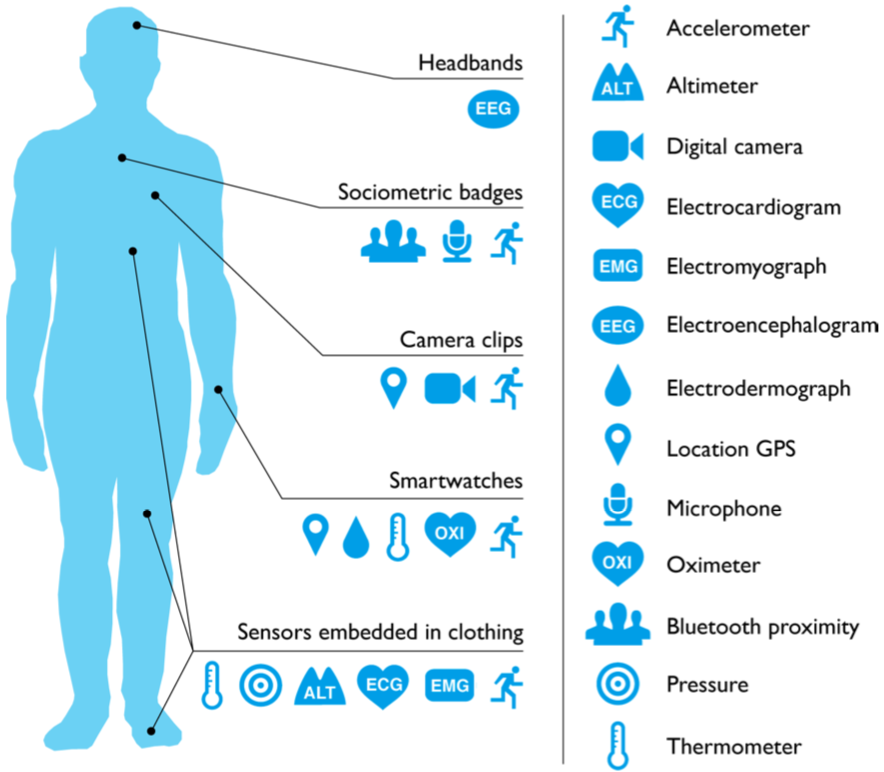
\includegraphics[width=10.5cm]{Thesis/data/sensoring.png}
		\caption{Health Wearables solution \cite{Wearables2016rise}}
		\label{fig:Wearables}
	\end{figure}
	
\end{itemize}
Both these approaches are obviously very useful to detect the state of health of the monitored person and they can be used together because one does not exclude the other. 

\section{Context-Modelling}
 There are several popular context modelling techniques, that are used in context-aware computing. The context models can be either dynamic or static and typically there are two different steps that could be distinguished to represent a context according to a model:
 \begin{itemize}
     \item Context modelling process: his function is triggered when a new context need to be defined in terms of characteristics, attributes, relationships with previously specified context, quality-of context attributes and the queries for synchronous context requests;
     \item Organize context according to the model: the result of the context modelling must be validated, then the new context information needs to be merged and added to the existing context information repository and finally make available the new context information when required;
 \end{itemize}
 
 
 \begin{figure}[h]
    \centering
    \begin{subfigure}{0.47\textwidth}
        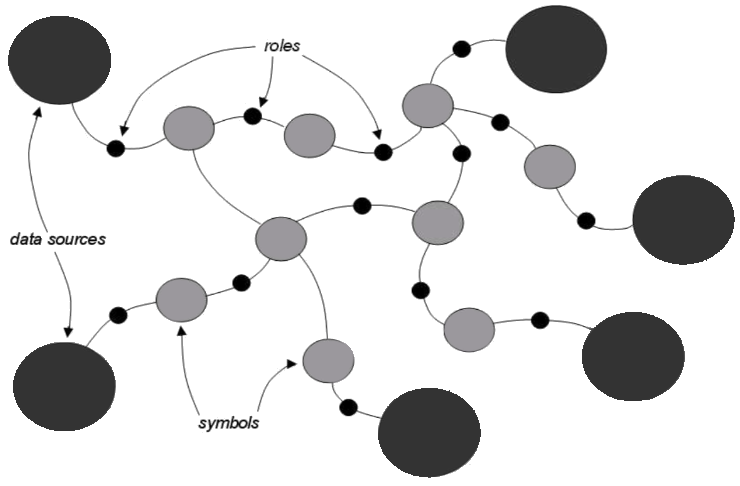
\includegraphics[width=\textwidth]{Thesis/data/ContextModelSketchh.png}
        \caption{A graphical sketch of the\\ proposed context model}
        \label{fig:sketch}
    \end{subfigure}
    \begin{subfigure}{0.47\textwidth}
        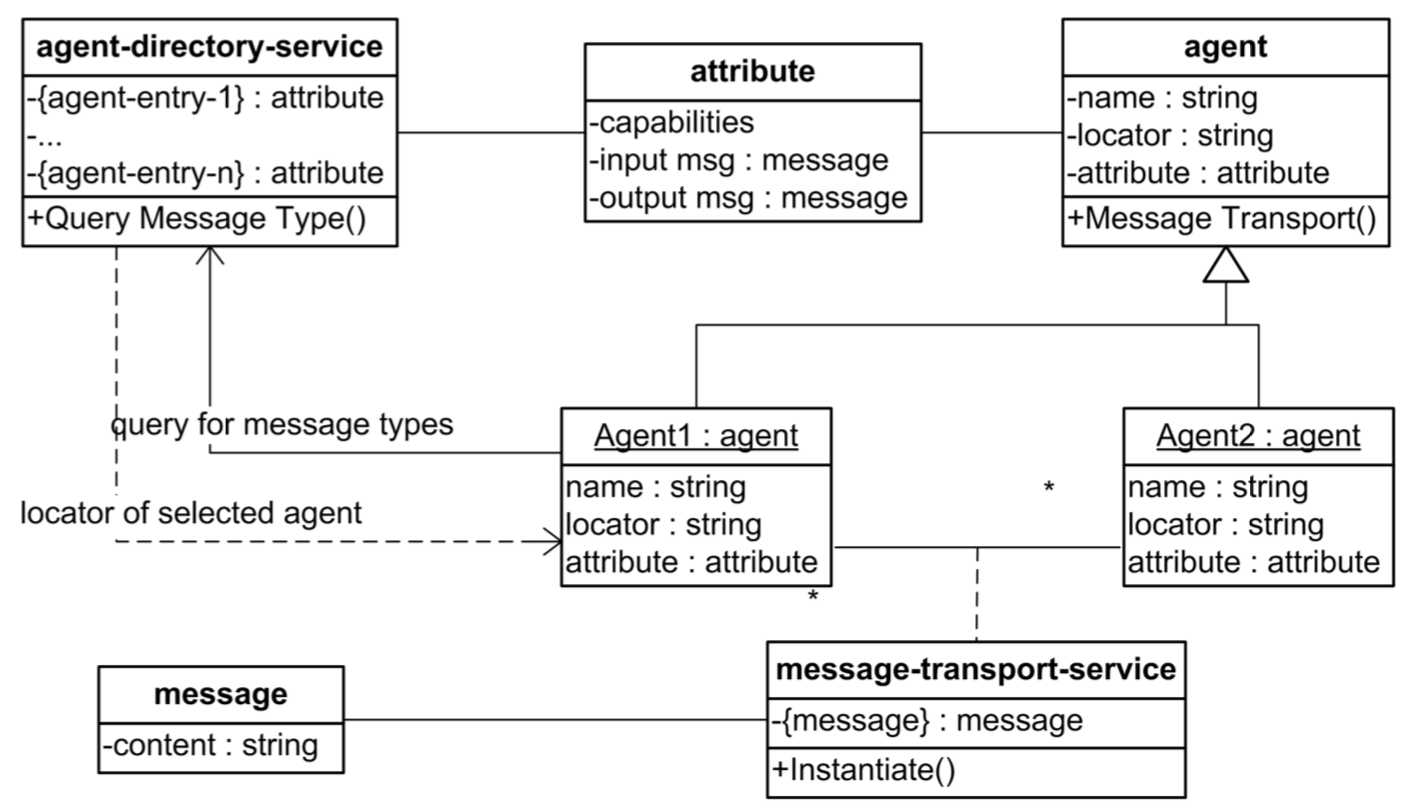
\includegraphics[width=\textwidth]{Thesis/data/architecture.png}
        \caption{A representation of the system architecture.}
        \label{fig:architecture}
    \end{subfigure}
    \caption{Context model sketch and system architecture representation}
    \label{fig:architecture-sketch}
 \end{figure}

 
 However the parameters and factors considered for the modelling context are very subjective. Indeed there is no standard to specify what type of information needs to be considered in the context modelling.
 
 Chen at al. \cite{chen2000survey} and Strang et al. \cite{strang2004context} discussed the most popular context modelling techniques, each of them having its own strengths and weaknesses that are synthetically shown in the table below \cite{perera2014context}.
 
 	\begin{figure}[H]
		\centering
		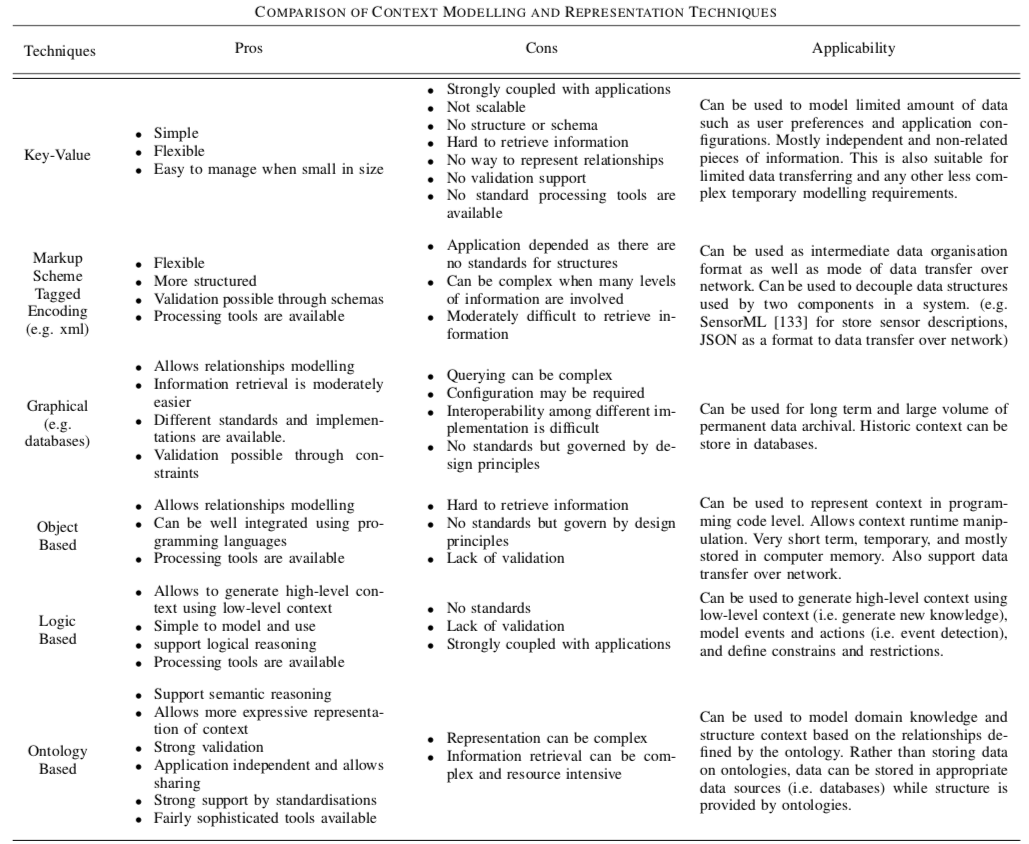
\includegraphics[width=17.5cm]{Thesis/data/ContextModelComparison.png}
		\caption{Comparison of Context Modelling and representation Techniques \cite{perera2014context}}
		\label{fig:populationProspect}
	\end{figure}
 As it will be better discussed in section \ref{ontology} the ontology, according to many surveys, is the preferred mechanism of managing and  modelling context, for all its advantages and despite its weaknesses \cite{perera2014context}.
 In fact it has several advantages, it separates domain knowledge from operational knowledge, shares a common understanding of the structure of information among people or software agents, and make domain assumptions explicit \cite{perera2014context}.
 
 
 \subsection{Reasoning}
 Context based reasoning can be considered as a method to deduce new knowledge based on the available context, indeed it can also be described as a process to provide high-level context deduction from a set of contexts \cite{perera2014context}.
 There are a lot of context reasoning decision models. Most of these models are not specific to context-reasoning but commonly employed in different fields such as machine learning or artificial intelligence \cite{perera2014context}.
 A survey paper \cite{perera2014context} has discussed solutions for context-reasoning, here briefly explained: 
 \begin{itemize}
     \item Supervised Learning: in this type of technique first we collect a training set examples. Then we label them according to the results we expect. Then we generate the expected results using the training data.
     They are commonly used where the feature set is easily identifiable;
     
     \textit{Artificial neural network, Bayesian Networks, Case-based reasoning, Decision tree learning, Support vector machines}
     \item Unsupervised Learning: they are used for situations where possible outcomes are not known. This type of solution has the great advantage of not needing training data;
     
     \textit{Clustering, k-Nearest Neighbour}
     \item Rule: applicable for situations where raw data elements need to be converted into high level context information. Suitable to use to define events , because it needs for few computational resources and storage. Simple to define and easy to extend; 
     \item Fuzzy Logic: applicable for situation where it is necessary convert low-level context in to more high-level context information. It is similar to probabilistic reasoning but confidence values represent degrees of membership rather than probability indeed in traditional logic theory, acceptable truth values are 0 or 1. In fuzzy logic partial truth values are acceptable \cite{perera2014context}; 
     \item Ontology based: It is mainly supported by two common representations of semantic web languages: RDF and OWL. Furthermore, it is based on description logic, which is a family of logic based knowledge representations of formalisms and it is used in case where knowledge is critical and it allows complex reasoning and complex representation basis on the ontology structure;
    
     \textit{First-Order Predicate Logic}
     
     \item Probabilistic logic: it allows decisions relying on probabilities attached to the facts related to the problem. It is commonly used where probabilities are known and combining evidence from different sources are essential. Indeed it can handle unseen situations and of uncertainty, combining the evidence; 
     
     \textit{Dempster-Shafer, hidden Markov Models, naive Bayes}
 \end{itemize}


\section{Ontology} \label{ontology}

According to \textit{Studer et al.} \cite{studer1998knowledge} an ontology is: 
\begin{center}
\textit{``A formal, explicit specification of a shared conceptualisation. A conceptualisation refers to an abstract model of some phenomenon in the world by having identified the relevant concepts of that phenomenon. Explicit means that the type of concepts used, and the constraints on their use are explicitly defined. For example, in medical domains, the concepts are diseases and symptoms, the relations between them are causal and a constraint is that a disease cannot cause itself. Formal refers to the fact that the ontology should be machine readable, which excludes natural language. Shared reflects the notion that an ontology captures consensual knowledge, that is, it is not private to some individual, but accepted by a group.”}
\end{center}


In the ontology based modelling the context is organized into ontologies with different semantic technologies, indeed there are several popular standards (RDF, RDFS, OWL) and reasoning capabilities usable depending on the requirement \cite{perera2014context}. 
In literature it is clear that the current recommendation, for semantic web ontology, is OWL 2 which is an extended version of OWL \cite{perera2014context}. The strength of OWL2 is that it adds more vocabulary for describing properties and classes, which could be used to build complex concepts starting with simpler concepts.
Furthermore, to get the real power of semantic technologies we also use SWRL rules in OWL because they are fully integrated into ontological reasoning. The cons of this approach is that ontologies can becomes exceedingly complex and too much computationally expensive, slowing down the reasoning process when the amount of data becomes larger and structure becomes too complex.

In conclusion there are several reasons to develop and use ontologies in contrast to other modelling techniques. The most common reasons are:
\begin{itemize}
    \item share a common understanding of the structure of information among people or software agents;
    \item analyse domain knowledge;
    \item separate domain knowledge from operational knowledge;
    \item high-level knowledge inferring;
    \item make domain assumptions explicit;
\end{itemize}


\section{ADL}
Our everyday activities tell us a lot about who we are and how we ensure a certain level of independence \cite{buoncompagni2017towards}. For this reason at first it is very important to define them. As early as late 1950s, we began the study of psychological, social and biological aspects of aging, analyzing the correlation between human actions and cognitive and motor capabilities \cite{buoncompagni2017towards}. 

The Index of Activities of Daily Living, described in \textit{``Multidisciplinary studies of illness in aged persons"} \cite{Multidisciplinary},  is the most used classification of functional status of elderly people and it is based on their ability to execute six different activities that are defined as ADLs:
%\begin{enumerate}[noitemsep,topsep=1pt,parsep=1pt,partopsep=1pt]
\begin{enumerate}
    \item \textit{bathing}
    \item \textit{dressing}
    \item \textit{toileting}
    \item \textit{transferring}
    \item \textit{continence}
    \item \textit{feeding}
\end{enumerate}

\begin{figure}[H]
	\centering
	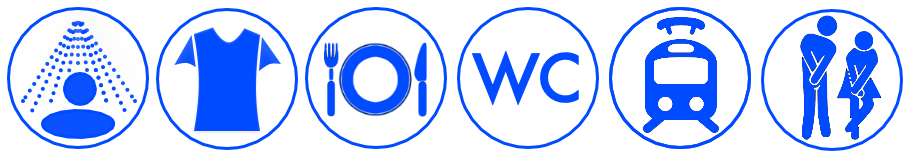
\includegraphics[width=17cm]{Thesis/data/IndexADL.png}
	\caption{Index ADL}
	\label{fig:indexADL}
\end{figure}

 These other nine activities, that take the name of Scale of Instrumental ADL \cite{lawton1970assessment} (IADL), require sufficient capabilities of social skills and planning capabilities using and interacting with everyday objects \cite{buoncompagni2017towards}. 
It takes into account 8 parameters, each parameter in turn can have different degrees of autonomy, for each degree of autonomy it is possible to attract the value 1 or the value 0, for a maximum total of 8 points. This concept can be summarized as shown in the table \ref{tab:IADL}. 

\subfile{IADL.tex}

At the end of the evaluation, by performing the sum of the values you can have a score that varies from 0 to 8.

The value 0 represents total dependence, while the opposite is total autonomy.

It is important to remember that if the non-exercise of an activity is not related to a loss of function but to the fact that that activity has never been performed even when the person was healthy and independent, that specific activity should not be considered to calculate the independence of a person.

%\begin{enumerate}[noitemsep,topsep=1pt,parsep=1pt,partopsep=1pt]
% \begin{enumerate}
%     \item \textit{placing a telephone call}
%     \item \textit{shopping}
%     \item \textit{preparing food}
%     \item \textit{housekeeping}
%     \item \textit{doing the laundry}
%     \item \textit{moving outdoor with public transports}
%     \item \textit{moving indoor on foot}
%     \item \textit{taking medications}
%     \item \textit{handling finances}
% \end{enumerate}

Nowadays, as explained in \cite{bruno2014public} the scale of IADL and the index of ADL are the \textit{de facto} standard indexes to evaluate person’s functional status\cite{buoncompagni2017towards}. 

In this essay the term ADL will assume a more general meaning, representing any  considered daily activities. 


\section{Human Activity Recognition}
There are many papers in literature where are discussed the automatic recognition of ADL. There are often differences about adopted sensing equipment or in the choice of the type of sensors, but typically all the solution share a common paradigm: ``\textit{distributed sensing, centralized reasoning}". The sensor information are distributed as raw data, with minimal or no processing, and made available to the reasoning system responsible for analyzing them to extract high level information, the ADL \cite{buoncompagni2017towards}.   

% A possible solution is to use binary sensors for their easy interpretation (eg: ON/OFF light switch) and their low cost. However, sensory information must be organized and analyzed in higher-level structures and this in literature, the most common and smart solution is doing it with \textit{ontologies}  already discussed in section \ref{ontology} \cite{buoncompagni2017towards}.

\section{Recognition Reliability} \label{reliability}
The reliability of the recognition is obviously fundamental for any system. Indeed we need to discriminate when a solution is consistent, when all the information is coherent or not with the specific activities detected, when there are some missing information or contradictory.
As explained by \textit{Sentz et al.} in \textit{Combination of evidence in Dempster-Shafer theory} \cite{sentz2002combination} to detail information about the confidence of the recognition, the reasoning module extends a hierarchy of coarse ontologies implementing the Dempster - Shafer (DS). 

However, there are also less extensive solutions, aimed at maximizing the accuracy of the recognition of a single type of ADL. Usually the solutions that follow this paradigm are based on a single or multiple homogeneous sensors that detect the quantities intrinsically correlated to a narrow range of activities. For example, the  water flow analysis in the house's plumbing system can accurately distinguish when a person is bathing or washing.

 \chapter{State of the art}
 
 \section{Arianna+} \label{Arianna}    
 In this Section, the objective will be to describe a knowledge-based approach for domain modeling (i.e., of context/activity) and reasoning (i.e., context/activity recognition), which is currently part of Arianna+ smart home framework \cite{kareem2018arianna}. \\
 Arianna is widely described by two papers \textit{Towards a new paradigm for assistive technology at home} of \textit{Buoncompagni et al.} \cite{buoncompagni2017towards} and \textit{Arianna+: Scalable Human Activity Recognition by Reasoning with a Network of Ontologies} of \textit{Yusha Kareem et al.} \cite{kareem2018arianna} I'll therefore avoid citing them to allow for a better reading. \\
 The approaches chosen and adopted by Arianna+ can be summarized as follows:
 \begin{itemize}
     \item Ontology Web Language (OWL), based on description logics (DL), allows to describe a given domain by defining relevant concepts (in the terminological box or TBox) and by asserting properties of individuals that are instances of those concepts (in the assertional box or ABox).
     Reasoners can then be used to derive facts, i.e., make implicit knowledge explicit, by reasoning mechanism \cite{donini1994deduction} based on \textit{subsumption} of concepts and \textit{instance checking};
     \item Rules based on the Semantic Web Rule Language extends the OWL axioms as follow:
    \begin{itemize}
        \item It includes a high-level abstract syntax for Horn-like rules which are of the form of an implication between an antecedent (body) and consequent (head). The intended meaning can be read as: whenever the conditions specified in the antecedent hold, then the conditions specified in the consequent must also hold \cite{horrocks2004swrl};
        
        i.e \texttt{Person(?p)} $\wedge$ \texttt{hasAge(?p,?age)} $\wedge$ \texttt{swrlb:greaterThan(?age,17)} $\rightarrow$ \texttt{Adult(?p)}
        
        \item SWRL is a rule language, not a query language. However, to extract information from ontologies a query language is needed to support querying of OWL ontologies are needed.
        This is possible by implementing built-in library using the standard SWRL built-in mechanism; 
        
         i.e \texttt{Person(?p)} $\wedge$ \texttt{hasAge(?p,?age)} $\wedge$ \texttt{swrlb:greaterThan(?age,17)} $\rightarrow$ \\  $\rightarrow$ \texttt{query:select(?p, ?age)}
        
    \end{itemize}
 \end{itemize}
 
  OWL-DL reasoners do not perform temporal reasoning due to issues of language expressivity. Nevertheless it is possible to bypass this limitation, indeed an ontology can acquire the symbolic temporal concept by hooking onto an upper ontology called OWLTime that provides concepts related to Allen’s temporal algebra which allows DL reasoners to consider instances of time belonging to particular intervals \cite{kareem2018arianna}.
  
  In the literature there are some attempts \cite{scalmato2013describing,buoncompagni2017towards}, of ontology-based AR, to take temporal reasoning into account accumulating temporal instances. Hence, their search space grows exponentially \cite{salguero2018using} with respect to the number of axioms in the ontology, which is an issue for real-time and large-scale,  applications. 
  To simplify, from now on in this text it will take basic temporal aspects for AR into account, without accumulating time instances within ontologies.

 
 In a real-world environment, it is crucial that AR systems must carefully guarantee \textit{scalability} and \textit{robustness} requirements \cite{kareem2018arianna}.
 \begin{itemize}
     \item The scalability can be achieved when the system is:
     \begin{itemize}
         \item modular with respect to the type of sensors, designing a system’s architecture that incorporates distributed sensors data;
         \item modular with respect to the activity models, designing them modularly as part of an ontology network, which is able to infer activities based on the occurrence of event;
         \item able to manage computational resources and memory, designing the activity models such that they represent the context over time, and evaluate them with the most suitable behaviour (e.g., with a scheduled frequency). Since they affect recognition performance in long-term applications 
     \end{itemize}
     \item The system’s robustness can be increased with redundancy of models with which we can assess the same activity;
 \end{itemize}
 
 
 \subsection{Activity Detection}
 \subsubsection{Dynamic Ontology Networks}
 In practice, Arianna+ corresponds to a network of ontologies tasked with a distributed reasoning process, each one dealing with different levels of detail in knowledge representation. 
 A fundamental step to reach this goal is  the definition of an activity model, its components and the procedures to evaluate it. In particular, Arianna+ describes each data sample through a generation time instant (T) and a fluent statement defined as a combination of a Boolean state (e.g., top $\top$ and bottom $\bot$).
 
 The recognition of an activity is represented as a new belief that acquires the Boolean $\top$ value by specifying the moment in which the execution of the activity is deduced.
 
 In this way, more complex models can be built as chains of sub-models, since their outcomes are statements, which can be embedded in more complex statements.
 This makes the Arianna+ reasoning engine scalable and suitable to validate different ways to assert the same abstract concepts.
 
Morover Arianna+ allows the use of simpler concepts to recognize several more complex concepts sharing the beliefs  with other models. For example, once the activity has been recognized as \textit{``cabinet door opened"}, it can be used to recognize an activity such as \textit{``leaving an object"} or \textit{``taking an object"} and both can be used to conclude that the person is \textit{``cooking"}.

 As already mentioned previously, Arianna+ grounds the above statement algebra formalization through a DL-based which allows for the specification of the \texttt{Statement} domain by restricting its instances to have exactly one property specifying its state and another specifying the generation time:
 
 \begin{equation}
     X \sqsubseteq_{=1} hasState(s_X) \sqcap_{=1} hasTime(t_X) \doteq Statement
     \label{statment}
 \end{equation}
 
 The ontology network is defined as a graph $G$, wherein the set of nodes $N$ are ontologies (each with an independent DL reasoner) containing statements of the form \ref{statment} and they are used to describe a specific part of the context, while the set of directed edges E are communication channels used for sharing statements between the nodes.
 
 Hence $G$ is of the form:
 \begin{equation}
     G = \left \{ N, E \right \}
 \end{equation}
 where, $N = n_1, n_2, ... , n_n$, so that each $node$ specializes in reasoning within a particular context, and $ E = e_{12},e_{13},...,e_{1n},e_{21},e_{23},...,e_{2n},...,e_{mn}$, so that the index of each $edge$ signifies the direction of flow of statements, e.g., in $e_{12}$ statements flow from $n_1$ to $n_2$. 
 
 The system checks the statements in the network with a given frequency and, when an event is detected, specific external procedures are executed in order to: (i) move statements from one node to another via edges, and (ii) evaluate models for activity recognition. For instance, statements could be generated from distributed sensors (e.g., detecting that Adam is in the kitchen at 8:00 am) and then the system aggregates this information with prior knowledge to detect events (e.g., Adam is in the kitchen in the morning). When such an event occurs, the model used for detecting that Adam is having breakfast is evaluated by checking statements and their temporal relations within the model.
 Moreover, activity models can generate statements, e.g., indicating that Adam had (or did not have) breakfast at a certain time, and hence can trigger new events, which can further be used to describe the context and evaluate models via procedure executions. A formal algebra of statements, used for defining events that execute procedures based on the context, has been proposed by \textit{Buoncompagni et al.} \cite{buoncompagni2017towards}.
 
 \subsubsection{A Network of Activity Detectors}
 To better understand the system let's try to consider a simplified ontology network $O$ as shown in \ref{fig:simplifiedOntologyNetwork}.
 Inside there are 6 nodes $n_i$ for $i=1,..,6$ where:
 \begin{enumerate}
    \item $n_1$ is a location-based contextualizing model called \textit{Place Ontology P};
    \item $n_2,...,n_6$ correspond to \textit{activity models} and can be called $A_j$ for $j=1,...,5$;
 \end{enumerate}
 
 Among these nodes we can therefore distinguish two types of statements where:
 \begin{enumerate}
     \item within $P$ only the spatial aspect is taken into account;
     \item within the $A_i$, both spatial and temporal aspects are taken into account;
 \end{enumerate}
 
  \begin{figure}[h]
	\centering
	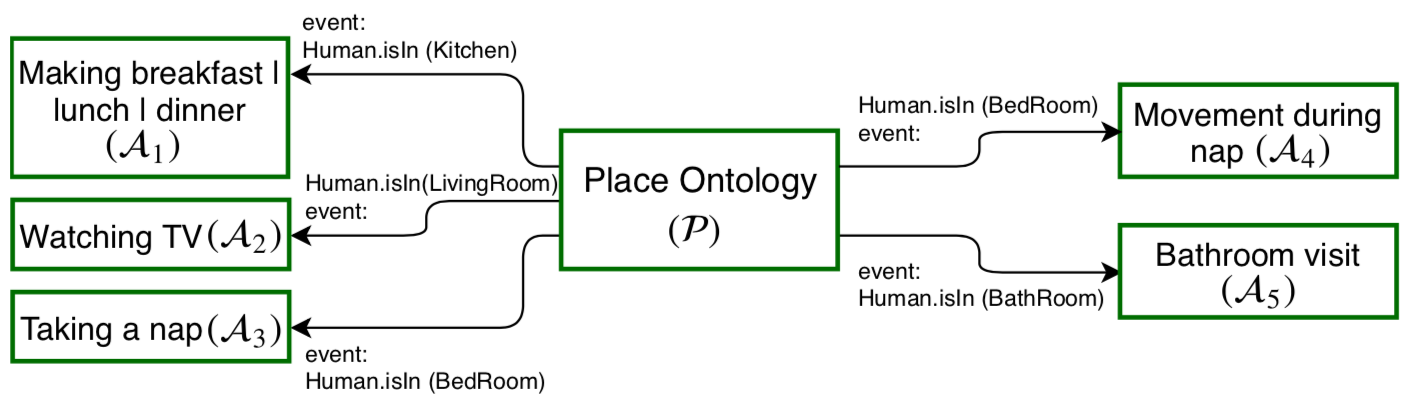
\includegraphics[width=15cm]{Thesis/data/O.png}
	\caption{A simplified ontology network $O$.}
	\label{fig:simplifiedOntologyNetwork}
  \end{figure}
   \begin{figure}[H]
	\centering
	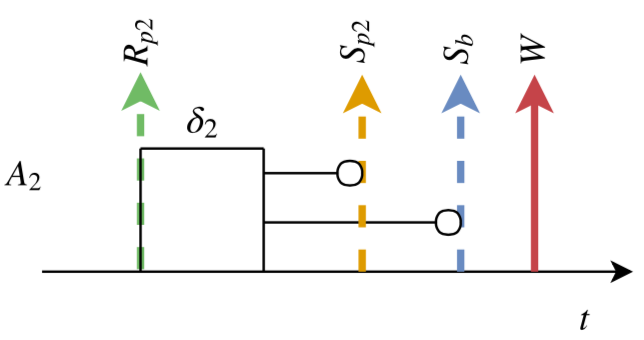
\includegraphics[width=8cm]{Thesis/data/event.png}
	\caption{``Visual representation of statements that make up the A2 model: statements are shown as vertical arrows where dashed arrows indicate information from $P$, and solid arrows indicate statements generated by this model. Statement indexes indicate sensors influencing the state of that statement, while the temporal restrictions are shown as black lines."}
	\label{fig:A2}
 \end{figure}

 The internal mechanisms between the nodes can be described as follows:
 \begin{itemize}
     \item activity models $A_i$ constantly waiting for $P$ to generate particular events;
     \item all the nodes communicating through the edges $E = e_{12}, e_{13}, e_{14}, e_{15}, e_{16}$;
     \item the instructions flow between the various nodes through the edges;
     \item the activities are activated when their independent reasoners check a particular event as shown in figure \ref{fig:simplifiedOntologyNetwork};
     \item a procedure generates a new declaration to notify the recognition of the activity when a model is satisfied;\\
     e.g. \texttt{WatchingTV.{hasState(True), hasTime(19:28)}}
 \end{itemize}

 To make sure that an activity is being recognized correctly, certain statements and temporal relationships must be satisfied.
 
 Considering the case A2 which recognizes the activity of figure \ref{fig:A2}:
 \begin{itemize}
     \item the arrows pointing upwards indicate a true state;
     \item the arrows pointing down indicate a false state;
     \item the arrows are dashed represent instructions from another node, in this case from $P$;
     \item the arrows are continuous when burns are generated by their own node, in this case by $A_2$;
 \end{itemize}
 
 ``In the Figure \ref{fig:A2}, we can see 4 statements: (i) statement $R_{p2}$, which is a dashed arrow of green color, is information coming from $P$; it signifies \texttt{isIn LivingRoom.{hasState(True), hasTime(19:25)}}, where the index $p2$ indicates that the sensor \texttt{PIR2} influences the state of this statement; (ii) statement $S_{p2}$, which is a dashed arrow of orange color, is information coming from $P$; it signifies that there is some motion in the living room after $\delta_2$ time units, naively representing the idea that, if Adam is sitting on the sofa then he is not sitting still; this statement can be replaced by a much robust statement, for instance, \texttt{sitting.{hasState(True), hasTime(19:26)}}, given that there may be other sensors in the system (e.g., wearable sensors, pressure sensors in the sofa); (iii) statement $S_b$, which is a dashed arrow of blue color, is information coming from $P$; it signifies \texttt{highBrightnessTV.{hasState(True), hasTime(19:28)}}, where the indexes $b$ indicates that brightness sensor influences the state of this statement; (iv) statement $W$, which is a solid arrow of red color, generated once the overall model is satisfied, it signifies \texttt{WatchingTV.{hasState(True), hasTime(19:28)}}; this happens when statements $S_{p2}$ and $S_b$ are generated after $\delta_2$ time units with respect to the $R_{p2}$ statement".
 

 It is important to note that when $A_i$ receives instructions from $P$, the values of the older instances get updated (if they are available), performing temporal reasoning using both symbolic relations (inferred by the DL reasoner) and numerical/logical operations on the timestamps (inferred externally). 
 After an activity is recognized, the statements are removed to reduce disk usage and the increasing complexity of the ontologies. 
 
 \subsection{Recognition Reliability}
 As explained in Section \ref{reliability} of the first Chapter, it is important to perform consistency checks to describe the context as a semantic hierarchy to be applied to statements over time.
 
 To do this Arianna+ uses the specifications of OWL API and Pellet to define semantic classes (indicated using capitalized names) and properties in their definitions (indicated with be/have characteristics), in order to allow the reasoner to classify individuals based on facts that have to be held true (in consistency terms) in the description of the environment.
 
 \subsection{Arianna+’s Architecture}
 In the Arianna+'s architecture we can distinguish sensing, aggregation, reasoning and application layer.  
 The ontology network $O$ is used over time to recognize activities based on the data taken from the database ($DB$), which stores the last values and timestamps coming from the aggregation layer which itself takes the data from the physical sensory layer.
 All the $DB$'s information are taken by the application layer to provide to the user a GUI to interact with.  
 
 \begin{figure}[H]
	\centering
	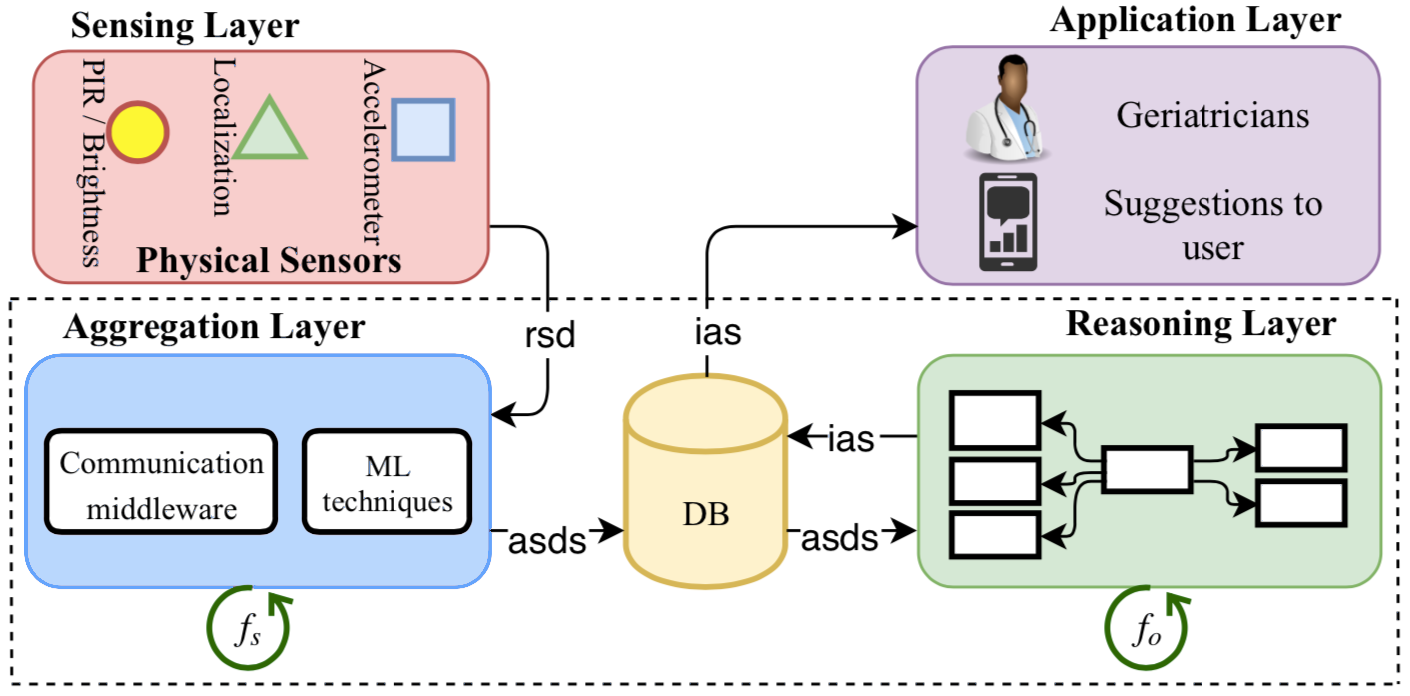
\includegraphics[width=17cm]{Thesis/data/layers.pdf}
	\caption{"Arianna+ ’s architecture where the link rsd signifies the flow of raw sensor data, asds signifies the flow of aggregated sensor data in the form of statements, ias signifies inferred activity statements and f signifies frequency. \cite{kareem2018arianna}"}
	\label{fig:layers}
 \end{figure}
 
 Now let's consider the tasks that the individual layers play:
 \begin{itemize}
     \item The \textit{reasoning layer} can be considered the core of Arianna+ in fact it corresponds to the ontology network where it is possible to distinguish two components:
     \begin{enumerate}
         \item initialization of the ontology network $O$ where the procedures and events are defined as edges and the TBox ontologies are defined as nodes;
         \item the frequency $f_o$ with which in the network the procedure $P$:
         \begin{itemize}
             \item takes the sensorial data aggregated from the database (link asds)
             \item updates the Box
             \item reasons (spatially) with the knowledge acquired in $P$
             \item declares an event if there is anyone;
         \end{itemize}
     \end{enumerate}
     Hence the event can thus activate the procedures of one or more activity models $A_i$. This procedure takes in statements from P and updates from its own ABox, then from the reasons for the recognition of a user activity.
     So if an activity is recognized, the procedure associated with the model saves the statement of the derived activity (link ias) in the database and if the update of the information corresponds to an event it can restart the process.
     
     Unfortunately, the time computation of the reasoning process is not negligible so if the frequency with which new data arrives is faster than the reasoning, the system would not meet the near real-time constraint.
     For this reason there is a control of this process dealing with the problem of computational complexity of the DL reasoner.
     
    \item The \textit{application level} is developed for two types of users:
    \begin{enumerate}
        \item for the geriatricians who can view statistics on the activities performed and explore further details such as vital signs and sleep quality;
        \item for the elderly person who could visualize suggestions based on his activities interfacing for instance through dialogue-based interfaces via virtual coaches;
    \end{enumerate}
    In addition, the database keeps track of $O$ statements so that medical or assistive staff can use or view them for additional services for the elderly.
    \item The \textit{aggregation layer} takes the raw sensors data from the detection level (link rsd), processes the raw data to generate statements in the form (\ref{statment}) to store them in the database (link asds). This level can therefore be considered an intermediary level of processing of the raw, which is based on classification modules (e.g., machine learning approaches) that allow to directly provide statements with semantics (e.g., sitting down).
    
    Moreover it is important to note that a statement with formal structure allows not only a modular approach to the evaluation of activities but also allows the system to take information from heterogeneous sensors. The whole process of elaboration can be more or less expensive from the point of view of computational time, for this reason according to the statement, not only must it consider the frequency with which the level of aggregation saves the information of the database but also the computational time required for the single module to aggregate the information.
 \end{itemize}
 
  The aggregation and reasoning layers are connected through the database where all the statements are stored, this is a means of communication between the two layers thus allowing 2 different work frequencies. In fact, the aggregation level stores the aggregated and updated information with a frequency $f_s$ while the reasoning layer bases its reasoning on the updated statements present in the $DB$ and taken every $\frac{1}{f_o}$ seconds.
 
 \section{Companion Robot}  \label{companionRobot}
 
 Most often for an elderly person, moving into to a retirement home is often caused by the loss of someone close or by the inability to look after themselves due to the decline of their health or lack of control over their lives.
 This means that the elderly at this stage of life loses certain aspects of their life that make them independent and satisfied.
 
 In fact, in nursing homes especially in the first phase of the stay, the elderly feel isolated, impotent and bored with the consequent risk of depression and loneliness.
 Unfortunately, even when they get used to staying in a nursing home, the feelings of loneliness and the isolation do not disappear because they are left with difficulty of establish new relationships \cite{assistiveRobots}.
 
 In the past, for an emotional support, many care homes incorporated animal visits, because they help fulfill criteria aimed at promoting better quality of life for the elderly by \cite{psicologicalEffects}:
 \begin{itemize}
     \item increasing social interactions;
     \item decreasing loneliness;
     \item countering boredom;
     \item helping foster a sense of purpose;
     \item helping to create social relationships;
 \end{itemize}
 Moreover, almost anyone, independent from their physical and cognitive damage, could interact with an animal.  \\
 In fact, interactions with animals have three effects \cite{psicologicalEffects}: 
 \begin{itemize}
     \item physiological effect (e.g. improvement of vital signs)
     \item psychological effect (e.g. improvement of mood and depression)
     \item social effect (e.g. facilitates communication)
 \end{itemize}

 The success of the animal is a fact, however unfortunately an animal needs care, and care staff of a nursing home must already take care of the elderly, therefore they often do not have the desire or time to take extra care of an animal.
 A robot companion on the other hand can have the same advantages as a real animal, yet no care or attention must be given to it because it is autonomous.
 In fact, the companion robots do not scratch or bite and don't host parasites or infectious diseases.
 
 In a study made in Japan, 14 residents who suffered from mild to moderate dementia were given the robot companion Paro. The results yieled an improvement in mood and depression and reduced stress levels; 
 The support staff defined the robot as a necessity because it made the elderly laugh and become more active by strengthening social ties.
 Unfortunately, studies like these are not solid because they generally take place within small samples and for a short period of time \cite{psicologicalEffects}.
 
 In assistive robotics we can distinguish different categories (fig: \ref{fig:layers}) \cite{assistiveRobots}:
 \begin{itemize}
     \item rehabilitation robots to help patients rehabilitate physical disabilities
     \item  Assisitive social robot:
     \begin{itemize}
         \item service type: it is not perceived as a social activity but as a support activity. In fact, it helps the elderly to remain or regain their independence in the functions of their every day and simultaneously allows the monitoring of their functions. (e.g.: artificial limbs)
         \item companion type: corresponds to the best solution for the health and psychological well-being of older users keeping company. For this type of robotic solution, the expressiveness of emotions during the interaction with the human is crucial.
     \end{itemize}
 \end{itemize}
 
 \begin{figure}[h]
	\centering
	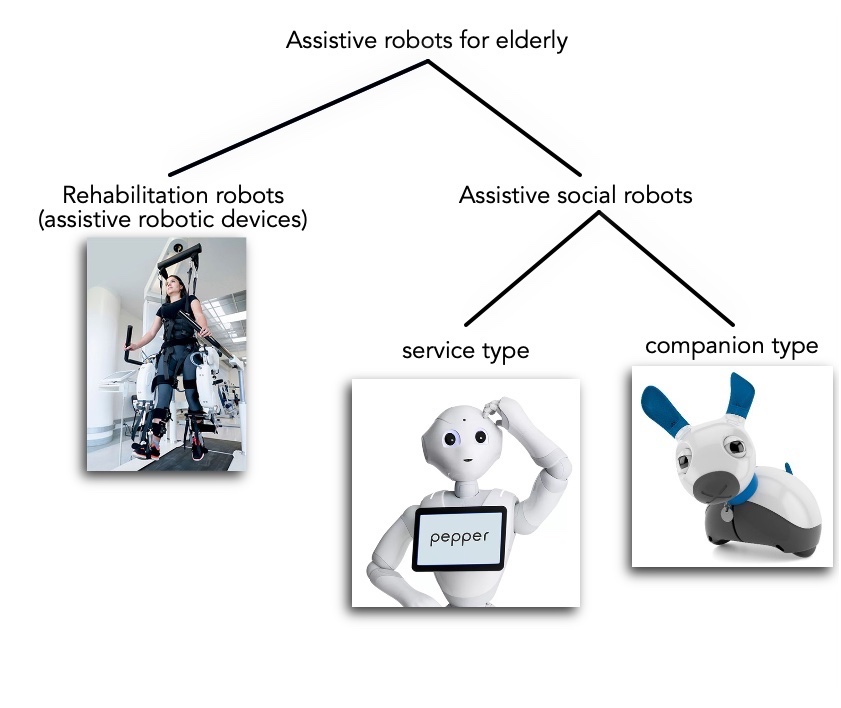
\includegraphics[width=14cm]{Thesis/data/TypeRobot.jpg}
	\caption{"Categorization of assistive robots for elderly" \cite{assistiveRobots}}
	\label{fig:layers}
 \end{figure}
 
 In assistive domotics, however, it is superfluous to distinguish between assistive and company robots because it is possible to combine both types in a single robotic solution. In fact, the robotic technology in eldcare hardly develops just to entertain.
 For example, a robot could be able to monitor the status of the elderly and keep them company helping to interact with other people and with technology.
 
 It is noteworthy that the use of a robot companion positively influences the acceptance of technology by the elderly and this is crucial if you want to insert the elderly into a smart home.
 
 In fact, the user considers the robot as a piece of technology with more or less easy to accept personality.
 Numerous studies have been done to ensure that above all, the elderly user is accepting of the technology.
 
 In technology acceptance models, enjoyment is sometimes incorporated as "Perceptual Enjoyment" which is defined as: "the extent to which the use of the system is perceived as enjoyable in itself, regardless of the consequences on performance that may be anticipated".
 
 In general, the acceptance of robots or intelligent agents takes place in terms:
 \begin{itemize}
     \item in term of usefulness and ease of use (functional acceptance)
     \item in accepting the robot as a conversational partner with which it can establish a Robot-Human relationship (social acceptance)
 \end{itemize}
 
 The first concept of a model of acceptance dates back to 1986 "Technology Acceptance Model for Empirically Testing New End-user Information Systems Theory and Results" which is still now the theoretical model among the most used in behavioral psychology \cite{davis1985technology,enjoymentModels}.
 It states, in its most basic form, that ease of use and perceived usefulness determine the behavioral intention of using a system.
 
 In 2003, \textit{Venkatesh et al.} published an inventory of all current models and factors and presented a new model called UTAUT \cite{venkatesh2003user,enjoymentModels}. It covers the following constructs :
 \begin{itemize}
     \item performance expectation
     \item effort expectation
     \item aptitude for the use of technology
     \item self-efficacy
     \item anxiety
 \end{itemize}
 
 As previously discussed, when it comes to accepting robots, it is important not only to direct acceptance in terms of ease of use and utility of a system, but also of relational or social acceptance. This means that a user accepts the robot as a conversational partner finding credible social skills in the robot, considering the robot as an autonomous social being. 
 
 From this we can conclude that regardless of the origin of the vocal interface, a conversational partner is crucial in the technological acceptance by the elderly. This topic is more widely described in the section \ref{speech}.
 
 In conclusion, we can summarize the advantages of using a robot companion in a smart nursing home:
 \begin{itemize}
     \item improves the health and psychological well-being of the elderly
     \item does not need treatment unlike a real animal
     \item can be used to monitor the elderly activities (in our case by Arianna+)
     \item helps the elderly accept technology
 \end{itemize}

 \section{Based dialogue management system} \label{speech}
 \subsection{Fields of study}
 The traditional telephone and video conference systems are examples of computer-human iterations focused on the terminal, in which the user focuses his attention and gaze, fixed on the terminal. So when deciding to start and then to end a call, we turn on or off our attention directed at the terminal. This type of iteration has more or less the same social characteristics as a formal face-to-face meeting \cite{augusto2010ambient}.
 Likewise in an environmental communication, as a person could dialogue with another person in another room, the same the dialogue management system can interact with the  user .
 
 The study of the interaction between human and technology in smart environments is studied by two complementary research sectors:
 \begin{itemize}
    \item the human-robot interaction (HRI) which can be defined as ``the study of humans, robots and the ways in which they influence each other". As a discipline, HRI concerns the analysis, design, modeling, implementation and evaluation of robots for human use.
    HRI is strongly related to human-computer interaction (HCI) and human-machine interaction (HMI). HRI, however, differs from HCI and HMI because it concerns systems (i.e. robots) that have more complex and dynamic control systems.
     
    \item social intelligence which, in its widest definition, is a person's ability to ``...get along with people in general, social technique or ease in society, knowledge of social matters, susceptibility to stimuli from other members of a group, as well as insight into the temporary moods of underlying personality traits of strangers." \cite{vernon1933some}.
 \end{itemize}

 both play an important role because they both study how much and with which dynamics man relates to the technological system, from the point of view of design and engineering in HRI and from the psychological point of view in social intelligence.

 \subsection{Approaches and advantages}
 There seem to be two views and probably complementary opinions about how humans interact:
 \begin{itemize}
     \item through a multitude of specific IT applications for each activity;
     \item through a centralized user interface which anticipates the needs of users through the adaptability of intelligence;
 \end{itemize}
 In the home domain, dialogue systems shall be required to appear as intermediaries between the systems embedded in the home and the people within them.
 In general, people in smart environments would like to be monitored as little as possible. Especially for the elderly it is necessary a trade-off between benefits and the intrusion into privacy. In fact, \textit{Portet et al.} have shown that the degree of acceptance of intrusive technology varies according to the severity of their disease \cite{portet2013design}. 
 Furthermore \textit{Saini et al.} demonstrated that providing a  of domestic dialogue system with social intelligence and behaviours ensures that the system is perceived as socially intelligent, leading to a more positive experience for users, who will be encouraged not only to accept the dialogue system but also the embedded technology \cite{saini2005benefits}.
 
 The advantages of a good interface are clear and well documented in the literature.
 For example, in a study conducted by \textit{Portet et al.} many opinions were collected concerning the appreciation of vocal interfaces in care homes for the elderly. In fact, 95\% of users would have continued to use this system even if it did not work perfectly and therefore occasionally made some mistakes \cite{portet2013design}.
 However, another important result emerging from these studies is that regardless of the technology used, no smart home application will be successful if it does not fit the individual user.
 In fact without an adequate assessment of the needs of the patient, the design of an interaction system, for the integration of new technologies, could be vain.
 
 So a system for human-machine and machine-man interaction, as a dialogue management system, must allow the user to interact as natural as possible. For that to happen it is necessary that the dialogue system not only correctly interprets the user's message but also places it in a given domain or context.
 
 In the case of implementation with Arianna+, it must be aware of the context in which the user located. In fact, if for example Arianna+ knows that the person is in the kitchen that there are the stove turned on and it is 8:15pm, it can conclude that it is cooking. Therefore any Arianna+ requests or intervention will be able to take account of context.

 To obtain such a result, the system must be adaptive, that is, it must be able to adapt not only to the context but also to the different operators with which it must communicate, adjusting its language and behavior according to needs.

 \subsection{Dialogue}
 By definition, dialogue is a communication process between two or more parts which requires sharing of context information. The style and the form of the dialogue can therefore vary according to the interlocutors and the context in which they are. In the same way, as a dialogue between a group of scientists in a laboratory is not the same of dialogue between teacher and her young student.
 However over the years it has been possible to determine many properties of dialogue are common to all.
 All the verbal communications between man and machine, computer or robot are made through an interface that according to Lansdale and Ormerod \cite{mccourt1996understanding} is controlled by 5 factors:

 \begin{itemize}
     \item \textit{linguistic competence} that is the ability to construct intelligible sentences and to understand the interlocutor speech. The dialogue between man and machine requires a vocabulary able to associate concepts with words or groups of these (eg: command words) and sequences of actions (grammar);
     \item \textit{conversational competence} is a crucial skill for any successful conversation. Unfortunately for the machine mechanisms like inference are much more complicated to adopt than to a person, who uses them without even noticing it. These, like other mechanisms, facilitate dialogue between people rather than a slower dialogue between man and machine. For this reason the user interface must be designed in such a way that users can unambiguously impart intentions and receive feedback;
     \item \textit{nonverbal skills} correspond to all those aspects of communication that concern the language of the body, in other words those gestures that add coherence to the dialogue. They act as adaptations and cues of control, providing information often redundant for a simpler and immediate understanding of the concept that one wants to express;
     \item \textit{medium constraints} correspond to the communication constraints imposed to the user to establish a dialogue, thereby implacably influencing the nature of the dialogue;
     \item \textit{task constraints} influence the structure of dialogue. In fact the lexicon as well as the structure of the language  varies depending on the context in which we are, to avoid misunderstandings and communicate complex information. In the same way as a military communication  will have a lexicon and a grammar completely different from a discussion between two people at the bar;
     
 \end{itemize}
 Factor not mentioned here but equally important is the experience. In fact, studies of experts have shown how the ability to assimilate and process information depends largely on the knowledge that you have of the topic. This is because the previous knowledge allows the experts to categorize and enclose more information in a single concept that instead may seem incomprehensible to a novice \cite{fong2001collaboration}.
 When a doctor starts a dialogue with a patient. The doctor initially takes control of the conversation, leading the dialogue to a sequence of questions and replies. On the other hand, when both interlocutors are experts in a specific subject matter, control of the conversation is shared by both parties.
 This dichotomy is presented in the same way in the interfaces with the user which or (1) guarantee to experts greater control than to novices (2) or ensure that the procedures, which the user is not able to do are, executed.

 \subsection{Dialogue management}
 Unless the interaction is elementary, with a fixed and limited grammar, the human-machine interface systems require dialogue management.
 The simplest function of dialogue management is to translate user requests so that the computer can understand it. An example is LUIS, a service offered by Microsoft based on machine learning techniques in which the machine is taught to interpret a voice input in a specific domain defining a priori a certain number of Entities and Actions. For example, with a voice input, "go to the kitchen" could return such as \texttt{"Entity"=kitchen} and \texttt{"Action"=move}, which information could be easily interpreted by the machine as part of its knowledge domain.
 In addition, however, the system must be able to manage the change of role that can take place at any stage of the dialogue. Dialogue management systems can allow the user, or computer, to take the initiative depending on the case. The difficulty lies in fact in dialogues where the initiative can be taken during any phase of the dialogue \cite{churcher1997dialogue}.

 There are two common methods for managing a dialogue:
 \begin{itemize}
     \item graphs: the dialogue consists of a series of nodes connected to each other where the user can choose which "to explore" (ex: "for reservations, press 2"). In this way the possibilities of choice are limited and therefore also the error;
     \item frames: database queries drive the dialogue ensuring less robustness compared to graphs but at the same time allowing greater flexibility for role switching;
 \end{itemize}
 
 \subsection{User Model}
 Given that dialogue should be studied on the basis of the interlocutor, it is important to define a model of them, so there is a reasonable mutual understanding. For example, the information presented (eg text, graphics), collections (eg: filtered, classic) can be adapted for the user. A profile or model of the user containing a set of information describing it. This information can therefore be used by the dialogue manager because typically a dialogue is strongly dependent on the properties of the interlocutor (eg: level of knowledge or skills, personal preferences, reactivity etc) \cite{fong2001collaboration}.
 Many of these properties can be attributed, for example, to social aspects, such as the place where they live. If for example the user is Japanese, they will have different customs from an American, together with different habits and different priorities. An efficient way to proceed is to define a generalization model, asking a small but targeted amount of information to the user. This makes it possible to define a generalized and stereotyped model that identifies the person within a sub-group properties that may be modified and added in successive phases \cite{fong2001collaboration}.

 \chapter{Conclusion}
 The goal of this study was to understand the main concepts of the environment as support for the elderly.
 First, an investigation was carried out to explore the main issues and concepts that govern ambient intelligence field.
 The most common techniques for modeling and determining a context have been defined showing the strengths and weaknesses of each possible approach. Based on the data collected, it was therefore decided to adopt the ontology-based approach.
 The work carried out also attempted to express the importance of the ADLs detection, which are fundamental daily activities in monitoring the patient's level of independence.
 
 The field of research is vast, as is the sample of choice among the different approaches. Above all, the number of different technologies required to make this kind of project adaptable and physically feasible within a real nursing home is vast. Just think about how to standardize all the information made available by the various devices scattered around the house, different in terms of type, brand, model and communication protocol.
 
 For this reason it was decided to choose a pre-existing architecture, Arianna +, already able to solve many of the problems listed above. This allowed me to focus on my real goals:
 -Give voice to our home so that it can not only be consulted, but capable of acting, addressing directly to the patient, in which case a situation is ambiguous in the eyes of the reasoning system.
 A vocal interface, however, is not only useful for this fact, as widely discussed in the [] section, it helps the elderly to accept the technological environment that surrounds it, allowing a simpler interaction.
 - Inserting a robot companion in the home environment, as discussed in the [] section, would improve the health and psychological well-being of the elderly by also helping them to accept the technology that surrounds and monitors them. Specifically, its use is essential to provide eyes to the home, making this invasion of privacy as acceptable as possible.
 
 
 L’obiettivo di questo studio è stato quello di capire i concetti principali dell'ambiente come supporto per anziani. 
Per prima cosa è stata svolta un’indagine per esplorare le principali tematiche e concetti che governano il mondo dell’ambient intelligence. 
Sono state definite le tecniche più comuni per modellare e determinare un contesto mostrando i pregi e i difetti di ciascun possibile approccio. Sulla base dei dati raccolti si è quindi deciso di adottare the ontology-based approach. 
Il lavoro svolto inoltre ha tentato di esprimere l’importanza del rilevamento delle ADLs, ovvero attività giornaliere fondamentali nel monitoraggio del livello di indipendenza del paziente.	

Il campo di ricerca è vasto, come il campione di scelta fra i diversi approcci. Ma soprattutto è vasto il numero delle diverse tecnologie necessarie affinchè un progetto di questo tipo sia adattivo e fisicamente realizzabile all'interno di una vera casa di cura. Basti solo pensare a come uniformare tutte le informazioni messe a disposizione dai diversi dispositivi sparsi nella casa, di diversi per tipologia, marca, modello e protocollo di comunicazione. 

Per questo motivo si è deciso di scegliere un'architettura pre-esistente, Arianna+, già in grado di  risolvere molte delle problematiche sopra elencate. Questo mi ha permesso di concentrarmi sui miei veri obiettivi:
-Dare voce alla nostra casa in modo che non solo possa essere interpellata, ma sia in grado di intervenire, rivolgendosi direttamente al paziente, nel qual caso una situazione risulti ambigua agli occhi del sistema di reasoning. 
Un'interfaccia vocale però non serve solo a questo infatti, come ampiamente discusso nella sezione [], aiuta l’anziano ad accettare l’ambiente tecnologico che lo circonda permettendogli una più semplice interazione.
	
- Inserire un companion robot in ambiente domestico, come discusso nella sezione [], migliorerebbe la salute e il benessere psicologico dell’anziano aiutandolo anche ad accettare la tecnologia che lo circonda e lo monitora.  Nello specifico il suo utilizzo è essenziale per fornire occhi alla casa, rendendo questa invasione della privacy il più accettabile possibile.

 
 
  
%  When dealing with rectangled triangles (see Figure \ref{triangle}) I sometimes used this theorem from \cite{pythm001}:
%  \begin{equation}\label{theo}
%   a^2 + b^2 = c^2
%  \end{equation}The demonstration is in Appendix \ref{sec:prooftheorem}.
 
%  \begin{figure}[h]\centering
%   \includegraphics[width=.5\linewidth]{triangle1}
%   \caption{A triangle with letters} \label{triangle}
%  \end{figure}
 
 
%  \chapter{Failed experiments}
 
%  When trying to draw a rectangled triangle, my program comes up with Figure \ref{triangle2} that is neither rectangled nor a triangle.
 
%   \begin{figure}[h]\centering
%   \includegraphics[width=.5\linewidth]{triangle2}
%   \caption{Triangle drawn by my program. Note the 4th side.} \label{triangle2}
%  \end{figure}
 
 
%  \chapter*{Conclusion}
%  \addcontentsline{toc}{chapter}{Conclusion}
 
 
 
%  % switch to A-B-C chaptering
%  \appendix	
 
%  \chapter{Proof of theorem \ref{theo}}
%  \label{sec:prooftheorem}
 
 
%  \begin{proof}
% \eqref{theo} was already demonstrated in \cite{euclides300}.
% \end{proof}
 
 \addcontentsline{toc}{chapter}{Bibliography}

 \bibliographystyle{IEEEtran}
 
 \bibliography{biblio}
 
 
 
 
\end{document}
